\section{Особенности задачи для данных из микроблогов}
\subsection{Основные характеристики данных}
Микроблоги -- это, в первую очередь, сервисы для упрощения публикации и восприятия пользовательских
данных. Обычно сообщения в микроблогах состоят из одного или пары предложений, а для Твиттера есть
строгое ограничение на длину твита -- 140 символов. В 140 символов пользователям платформы необходимо
уместить контекст, своё отношение к теме и, возможно, ссылку на фотографию, Интернет-ресурс или
другой медиа объект. Часто контекст восстанавливается из окружающего мира, то есть пользователь
пишет о том, что волнует Интернет в этот момент, и люди, владея этой информацией, сопоставляют
высказывание с реальными событиями. У компьютера так просто быть в курсе обсуждаемых тем не
получается, поэтому на восстановление контекста рассчитывать не приходится.

Платформы для ведения микроблогов также являются социальными сетями, где пользователи могут
взаимодействовать друг с другом. В Твиттере, например, кроме социальных графов можно наблюдать
графы, в которые выстраиваются сами сообщения: пользователи могут отвечать на твиты, а также
размещать у себя твиты других пользователей, в терминологии платформы это называется
``ретвитить''. Информация о социальных взаимодействиях может уточнять результаты классификации,
например, есть интуитивное предположение, что ответ на отрицательно окрашенное сообщение тоже
попадёт в класс негативных.

\subsection{Особенности текстов}
\subsubsection{Смайлы}
Для выражения эмоций в тексте пользователи ставят смайлы. Смайл -- это набор символов, условно
иллюстрирующий выражение лица автора, а точнее его настроение. Все смайлы можно поделить на
восточные и западные по географии их использования, последние приведены в таблице \ref{tab:smileys}
с метками, соответствующими их эмоциональной окраске. В случае с короткими текстами нет более
простого способа отметить своё отношение к теме, чем поставить смайл, но не все пользователи так
делают, поэтому размечать сообщения с их помощью в общем случае не получится. Есть и более сложные
конструкции из скобок, двоеточий и других симовлов, но они используются не так часто и обычно
означают уже не просто отношение, а какие-то действия или объекты, то есть эмоциональной окраски не
несут.

\begin{table}[h]
\begin{tabular}{|cc|cc|cc|cc|cc|}
\hline
\textbf{Смайл}              & \textbf{Метка} & \textbf{Смайл}         & \textbf{Метка} & \textbf{Смайл}   & \textbf{Метка} & \textbf{Смайл} & \textbf{Метка} & \textbf{Смайл} & \textbf{Метка} \\ \hline
:-)                         & +              & :)                     & +              & :o)              & +              & :{]}           & +              & :3             & +              \\
:c)                         & +              & :\textgreater          & +              & ={]}             & +              & 8)             & +              & =)             & +              \\
:\}                         & +              & :\textasciicircum )    & +              & :>)              & +              & :-D            & +              & :D             & +              \\
8-D                         & +              & 8D                     & +              & x-D              & +              & xD             & +              & X-D            & +              \\
XD                          & +              & =-D                    & +              & =D               & +              & =-3            & +              & =3             & +              \\
B\textasciicircum D         & +              & :-))                   & +              & \textgreater:{[} & -              & :-(            & -              & :(             & -              \\
:-c                         & -              & :c                     & -              & :-\textless      & -              & :>C            & -              & :\textless     & -              \\
:-{[}                       & -              & :{[}                   & -              & :\{              & -              & ;(             & -              & :-||           & -              \\
:@                          & -              & \textgreater:(         & -              & :’-(             & -              & :’(            & -              & :’-)           & +              \\
:')                         & +              & D:\textless            & -              & D:               & -              & D8             & -              & D;             & -              \\
D=                          & -              & DX                     & -              & v.v              & -              & D-‘:           & -              & :*             & +              \\
:\textasciicircum *         & +              & (                      & +              & \}\{            & +              & )              & +              & ;-)            & +              \\
;)                          & +              & *-)                    & +              & *)               & +              & ;-{]}          & +              & ;{]}           & +              \\
;D                          & +              & ;\textasciicircum )    & +              & :-,              & +              & \textgreater:P & +              & :-P            & +              \\
:P                          & +              & X-P                    & +              & x-p              & +              & xp             & +              & XP             & +              \\
:-p                         & +              & :p                     & +              & =p               & +              & :-Þ            & +              & :Þ             & +              \\
:þ                          & +              & :-þ                    & +              & :-b              & +              & :b             & +              & d:             & +              \\
\textgreater:\textbackslash & -              & \textgreater:/         & -              & :-/              & -              & :-.            & -              & :/             & -              \\
:\textbackslash             & -              & =/                     & -              & =\textbackslash  & -              & :L             & -              & =L             & -              \\
:S                          & -              & \textgreater.\textless & -              & :|               & -              & :-|            & -              & :\$            & -              \\
O:-)                        & +              & 0:-3                   & +              & 0:3              & +              & 0:-)           & +              & 0:)            & +              \\
0;\textasciicircum )        & +              & O\_O                   & -              & \o/              & +              & \textless3     & +              & \textless/3    & -              \\ \hline
\end{tabular}\caption{Эмоциональная окраска смайлов.}\label{tab:smileys}
\end{table}

\begin{figure}[h]
\centering
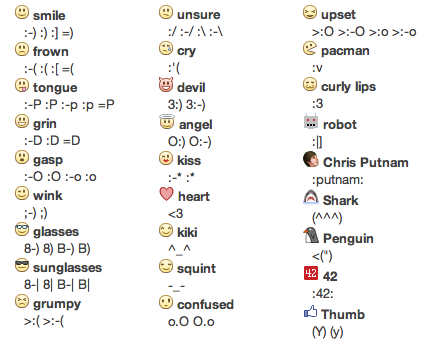
\includegraphics[width=0.5\textwidth]{ListofFacebookChatEmoji}
\caption{Некоторые графические смайлы, используемые в Facebook.}
\label{emoji}
\end{figure}

\pagebreak
Кроме ASCII смайлов есть ещё и графические -- это картинки, которые вставляются в текст. В
современных веб-сервисах и мобильных приложениях используется графический язык Emoji\footnote{www.emoji-cheat-sheet.com} для
записи слов, эмоций и действий. На рисунке \ref{emoji} изображены некоторые известные графические
смайлы, которые используются в социальной сети Facebook\footnote{facebook.com}. Обычно для
каждого из них есть ASCII аналог, причём не один. Набирая сообщение на клавиатуре компьютера или
ноутбука, удобнее поставить двоеточие со скобкой, но смартфоны и планшеты предоставляют все удобства
для вставки улыбчивых картинок: наряду с русской и английской клавиатурой, например, на них можно
подключить и клавиатуру графического языка Emoji.

Так как смайлы являются своего рода разметкой сообщений самими пользователями, их необходимо
использовать при анализе эмоциональной окраски. В этой работе будет рассмотрено применение
символьных и графических улыбок для сбора корпуса твитов и для предобработки данных непосредственно
перед классификацией.

\subsubsection{Хештеги}

Ещё одна особенность общения в микроблогах -- хештеги. Пользователь помечает в своём сообщении
слово, ставя перед ним ``\#'', тем самым показывая связь объекта, обозначаемого этим словом, и всего
твита. Платформы для микроблогов предлагают возможность искать по хештегам, выбирать из них
популярные и следить за потоками актуальной информации. Многие хештеги используются в течение
короткого периода времени, но затем именно по ним можно найти информацию, которая когда-то была
актуальной и понадобилась через несколько месяцев. Например, организаторы мероприятий стараются
придумывать уникальный хештег, размещать его на информационных стендах, чтобы участники следили за
твитами друг друга и распространяли информацию по всему Интернету. Можно сказать, что это
повествовательная функция хештегов, точнее, тех из них, которые указывают на объект,~-- они могут
помочь осуществлять поиск сообщений на определённую тему.

Другую функцию этих специальных слов-ассоциаций можно назвать описательной. Именно такие хештеги
можно использовать в определении эмоциональной окраски текстов. В работе
\cite{qadir2013bootstrapped} предложен способ классифицикации хештегов по их эмоциональной
окраске. Авторы предлагают читателям посмотреть на 20 самых популярных хештегов из каждой
группы. Для наглядности в таблице \ref{tab:hashtags} приведены первые пять для каждой эмоции.

\begin{table}[h]
  \begin{tabular}{|c|c|c|c|c|} \hline
    \textbf{Привязанность} & \textbf{Ярость} & \textbf{Страх} & \textbf{Наслаждение} & \textbf{Грусть}\\ \hline
    \#youthebest&\#godie&\#hatespiders&\#thankinggod&\#catlady\\
    \#yourthebest&\#donttalktome&\#freakedout&\#thankyoulord&\#buttrue\\
    \#hyc&\#fuckyourself&\#creepedout&\#thankful&\#singleprobs\\
    \#yourethebest&\#getoutofmylife&\#sinister&\#superexcited&\#singleproblems\\
    \#alwaysandforever&\#irritated&\#wimp&\#tripleblessed&\#lonelytweet\\
    \hline
  \end{tabular}
  \caption{Самые популярные хештеги для пяти чувств: привязанности, ярости, страха, наслаждения и
    грусти. }\label{tab:hashtags}
\end{table}

Использование хештегов непосредственно для оценки эмоциональной окраски можно считать примерно таким
же, как и у смайлов, но лишь тогда, когда слово однозначно относится либо к положительным,
либо к отрицательным. В противном случае они либо становятся обычными словами: без символа ``\#''
они участвуют в классификации наравне с другими, либо уточняют вероятность сообщения попасть в тот
или иной класс при помощи подсчёта условных вероятностей, где условием и является хештег.

\subsubsection{Сокращения, пролонгирования и пунктуация}
Тексты в микроблогах содержат не только уточняющую информацию, но и отчасти мешающую. Её нужно научиться использовать, так как
специфика сообщений не позволяет хоть что-то выкидывать.

Ограничение в 140 символов заставляет людей сокращать слова, причём как при помощи общеизвестных
аббревиатур, например, ``СПбГУ'' -- это Санкт-Петербургский Государственный Университет, так и при
помощи жаргонных конструкций: ``h8'' -- это на самом деле hate. На примере последнего видно, что
избавиться от этого слова было бы расточительно, но вряд ли ``h8'' внесло бы вклад в
вероятность сообщения попасть в класс отрцательных такой же, как и слово ``hate''. Получается,
сокращения нужно уметь переводить.

Когда пользователям кажется, что длина сообщения не такая уж и маленькая, они используют
пролонгирования гласных -- ещё один способ выражать обеспокоенность темой твита. Автор преумножает
гласную в слове, изображая её продолжительное звучание, то есть, например, крик. Так ``nooooooo''
будет, скорее всего, означать категорическое несогласие, а ``so cuuuute'' -- умиление. Таким
образом, каждое такое слово что-то значит, но классификатор может об этом не знать, значит, нужно
рассказывать классификатору какими-то другими способами, что это важное слово и какое из известных
является его менее эмоциональным аналогом.

Авторская пунктуация может рассказать об эмоциональной окраске сообщения не меньше, чем
смайлы. Например, в нейтральных твитах крайне редко встречаются восклицательные знаки. Впрочем,
однозначно классифицирующих особенностей пунктуации не так и много: наличие восклицательных знаков
указывает на наличие эмоциональной окраски, при этом нельзя без дополнительного анализа сказать,
какой именно; сочетание ``?!'', скорее всего, будет означать недоумение, то есть классифицируется
как отрицательное; многоточия обычно говорят о нейтральности.

\subsection{Использование особенностей текстов для предобработки}\label{spec}
Смайлы, хештеги, сокращения, пролонгирования и пунктуация -- это то, про что классификатор уже не
знает, то есть перед подачей ему сообщения необходимо преобразовать это сообщение так, чтобы все
перечисленные особенности не выбивались и превратились в обычные слова.

Смайлы, перечисленные в таблице \ref{tab:smileys}, заменяются в тексте на соответствующую им
метку. Это делается для того, чтобы в обучающей выборке слово ``+'' встретилось больше раз среди
положительных твитов, тем самым, в вероятность попасть в класс положительных ``+'' даст больший
вклад, чем  просто ``:)''. Так же, заменой на ``+'' и ``$\minus$'', обрабатывается пунктуация.

К смайлам, заменяемым на метки, добавляется замена некоторых однозначно классифицирующихся
хештегов. Происходит это по той же причине, что и со смайлами. Если замена хештега не произошла, то
считается, что он должен стать обычным словом, то есть ``\#'' из начала пропадает, и дальше работа
происходит уже без учёта того, что это хештег.

Если в сообщении встречается неизвестное слово, его стоит проверить на наличие в словаре сокращений. В данной
работе используется словарь ``No slang''\footnote{http://www.noslang.com/}, к которому программа
обращается во время подготовки данных к подаче классификатору. Запрос к словарю происходит в
онлайн-режиме, и для обработки сокращений нужно подключение к Интернету.

Повторения гласных убирать совсем не нужно: достаточно сократить количество повторяющихся гласных
до двух, то есть ``nooooooo'' заменится на ``noo''. В этом случае слово ``noo'' может встретиться в
обучающей выборке, в отличие от ``nooooooo'', где именно семь, а не восемь или девять букв
``о''. Таким образом слово ``no'' уже не то же самое, что ``noo'', но все, сколько угодно длинные
продолжения гласной ``о'' сведутся к одному и тому же эмоциональному ``noo'', которое даст каждому
из таких слов с продолжениями одинаковый повод попасть в класс ``$\minus$''.
